\documentclass[aps,prx,reprint,amsmath,amssymb,floatfix,nofootinbib,superscriptaddress]{revtex4-2}

\usepackage{graphicx}
\usepackage{dcolumn}
\usepackage{bm}
\usepackage{hyperref}
\usepackage{booktabs}
\usepackage{array}
\usepackage{xcolor}

\hypersetup{
  colorlinks=true,
  linkcolor=blue!50!black,
  citecolor=blue!50!black,
  urlcolor=blue!50!black,
  pdftitle={Leggett-Garg saturation and structural signatures in Fibonacci-anyon braiding},
  pdfauthor={Berkay Yuksel Sayim},
  pdfkeywords={Leggett-Garg inequality, Fibonacci anyons, non-abelian braiding,
               macrorealism, Luders bound, topological quantum computation,
               modular tensor category, universality}
}

\begin{document}

\title{Leggett-Garg saturation and structural signatures in Fibonacci-anyon braiding}

\author{Berkay Y\"uksel Sayim}
\email{sayim.berk@gmail.com}
\affiliation{Independent researcher\\
\href{https://orcid.org/0009-0004-4993-7352}{ORCID: 0009-0004-4993-7352}}

\date{\today}

\begin{abstract}
We numerically test the three-time Leggett--Garg inequality
$K_{3} \leq 1$ for the standard B$_{3}$ Fibonacci-anyon braiding
representation on the two-dimensional fusion space of three $\tau$ anyons.
Exhaustive enumeration over all $4^{L}$ braid words up to length $L=11$
and random sampling to $L=40$ show that $K_{3}$ saturates the L\"uders
bound $3/2$ to $99.998\%$, with the first violation already at $L=3$.
Three structural signatures accompany the saturation. First, replacing
the Fibonacci generators by the Ising-anyon generators on the same
$2$D fusion space gives $K_{3}=1$ exactly for every $L \leq 40$ and every
random word tested---a sharp split that mirrors the Hou--Shtengel
no-Bell-violation result for Ising braiding in the spatial CHSH setting.
Second, the sector phase $\delta$ tunes a singular point
$\delta = 3\pi/5$ at which the generator $\sigma_{1}$ collapses to a
scalar to machine precision and braiding becomes impossible.
Third, the Fourier spectrum of $K_{3}(\delta)$ is dominated by the
$2\pi/6$ harmonic, reflecting the six R-matrix insertions per
$(\sigma_{1}\sigma_{2})^{3}$ word rather than the $\mathrm{Z}_{5}$
period of the central element. We also find that $K_{3}$
at the optimal $L=11$ word is initial-state independent: every pure
state and the maximally mixed state give the same value to $10^{-16}$.
All Yang--Baxter, unitarity, and $(\sigma_{1}\sigma_{2})^{3}$-scalar
sanity checks pass at machine precision. To our knowledge this is the
first Leggett--Garg test for non-abelian anyon braiding specifically,
and for the Fibonacci model in particular. The only previously
published ``Leggett--Garg on a topological system'' is
G\'omez-Ruiz \emph{et al.} (2018), which differs in three ways: the
system is abelian (Kitaev chain, not Fibonacci); the qubit basis is
formed by paired edge Majorana modes rather than the fusion channel
of three anyons; and $K_{3}$ is used as a probe of a topological
phase transition rather than as a saturation test. Code,
seeds, and data are released with the preprint.
\end{abstract}

\maketitle

\section{Introduction}

The Bell inequalities probe whether spatially separated subsystems can
be described by a joint local-realistic distribution; the
Leggett--Garg inequalities~\cite{LeggettGarg1985} probe the temporal
analogue---whether a single system carries a definite value of an
observable between measurements, independent of whether it is measured
(``macrorealism''). For three projective measurements of a dichotomic
observable $Q \in \{+1,-1\}$ at times $t_{1} < t_{2} < t_{3}$, with
two-time correlators $C_{ij} \equiv \langle Q(t_{i})\,Q(t_{j}) \rangle$,
the simplest combination
\begin{equation}
  K_{3} \;=\; C_{12} + C_{23} - C_{13}
\end{equation}
satisfies $K_{3} \leq 1$ under macrorealism, $K_{3} \leq 3/2$ under
L\"uders projective quantum measurement on a two-level system (the
``temporal Tsirelson bound''~\cite{Budroni2014}), and $K_{3} \leq 3$
algebraically.

Non-abelian anyons are the natural laboratory for asking whether a
\emph{topological} two-level system---a fusion-channel qubit whose
algebra has no tensor-product factorization into spatial
subsystems~\cite{NayakSimonStern2008}---also saturates the L\"uders
bound. The Fibonacci anyon model is the smallest model in which
braiding alone is computationally universal (dense in $\mathrm{SU}(2)$
on the relevant fusion space), while the Ising model, including its
Majorana-zero-mode realizations, gives only the Clifford group and is
provably unable to violate the spatial CHSH inequality without an
additional non-Clifford gate~\cite{HouShtengel2016}. The two models
therefore form a natural \emph{universality split}: a property that
requires arbitrarily close approximation of generic unitaries should
discriminate sharply between them.

The temporal counterpart has not been measured. The only published
``Leggett--Garg on a topological system'' is G\'omez-Ruiz
\emph{et al.}~\cite{GomezRuiz2018}, who tested $K_{3}$ for Dirac
qubits formed from edge Majorana modes of the abelian Kitaev chain.
We state up front how the present work differs, because this
demarcation defines the novelty claim:

\begin{center}\small
\begin{tabular}{lll}
\toprule
                       & G\'omez-Ruiz 2018~\cite{GomezRuiz2018} & this work \\
\midrule
anyon type             & abelian (Kitaev chain) & \textbf{non-abelian} (Fibonacci) \\
qubit basis            & paired edge Majoranas  & \textbf{$3\tau$ fusion channel} \\
universal braiding?    & no (Clifford)          & \textbf{yes} (dense in $\mathrm{SU}(2)$) \\
role of $K_{3}$        & phase-transition probe & \textbf{saturation test} (L\"uders) \\
saturation reported    & no                     & \textbf{$99.998\%$} of $K_{3}=3/2$ \\
\bottomrule
\end{tabular}
\end{center}

\noindent The two papers are methodologically and physically distinct
sub-cases of ``Leggett--Garg on a topological system''. The
non-abelian Bell/Leggett--Garg literature for Fibonacci or Ising
anyons is otherwise empty; Brennen \emph{et al.}~\cite{Brennen2009}
construct explicit CHSH-violating settings on the Fibonacci/Ising
fusion spaces, but do not test the temporal inequality. Recent
solid-state and quantum processor demonstrations of non-abelian
topological order~\cite{Andersen2023,Iqbal2024,Xu2024,Minev2025}
provide a plausible target for an experimental test but have not yet
been used for one.

We present the simplest possible numerical setup for the temporal
question. Section~\ref{sec:setup} fixes the generators, correlator,
and sanity checks. Section~\ref{sec:results} reports five connected
findings: (i)~Fibonacci L\"uders saturation to $99.998\%$;
(ii)~an exact $K_{3}=1$ for Ising at every length tested;
(iii)~an algebraic scalar-singularity point $\delta = 3\pi/5$;
(iv)~a $2\pi/6$ dominant Fourier period of $K_{3}(\delta)$,
algebraically tied to the six R-matrix insertions per
$(\sigma_{1}\sigma_{2})^{3}$ word;
(v)~complete initial-state independence of the optimal $K_{3}$.
Section~\ref{sec:discussion} relates the universality split to the
known CHSH split and lists what the results do \emph{not} say.

\section{Setup}
\label{sec:setup}

\subsection{Fusion space and observable}

We work on the two-dimensional fusion space of three $\tau$ anyons
with total charge $\tau$ in the Fibonacci modular tensor
category~\cite{NayakSimonStern2008}, identified with the standard
B$_{3}$ Burau-Jones representation. The dichotomic observable
$Q = \sigma_{z}$ corresponds to a measurement of the topological
charge of an anyon pair~\cite{Bonderson2008}; experimentally this is
the interferometric fusion outcome of the pair.

\subsection{Generators}

We use the standard Fibonacci $F$- and $R$-symbols~\cite{NayakSimonStern2008}:
\begin{equation}
  F \;=\;
  \begin{pmatrix} 1/\varphi & 1/\sqrt{\varphi} \\
                  1/\sqrt{\varphi} & -1/\varphi \end{pmatrix},
  \qquad
  R_{1} = e^{-4\pi i/5}, \quad R_{\tau} = e^{+3\pi i/5},
\end{equation}
with $\varphi = (1+\sqrt{5})/2$, giving
\begin{equation}
  \sigma_{1} \;=\; \mathrm{diag}(R_{1},\,R_{\tau}\,e^{i\delta}),
  \qquad
  \sigma_{2} \;=\; F\,\sigma_{1}\,F.
\end{equation}
Here $\delta$ is an algebraic phase-deformation parameter: $\delta=0$
recovers the standard Fibonacci theory. The braid alphabet is
$\{\sigma_{1},\sigma_{1}^{-1},\sigma_{2},\sigma_{2}^{-1}\}$.

The Ising data~\cite{NayakSimonStern2008} on the analogous $2$D
fusion space are
\begin{equation}
  F_{\mathrm{I}} \;=\; \tfrac{1}{\sqrt{2}}
  \begin{pmatrix} 1 & 1 \\ 1 & -1 \end{pmatrix},
  \qquad
  R^{\sigma\sigma}_{1} = e^{-i\pi/8},
  \quad
  R^{\sigma\sigma}_{\psi} = e^{+i 3\pi/8},
\end{equation}
with $\sigma_{1},\sigma_{2}$ constructed identically; this is the
non-universal Clifford branch.

\subsection{Correlator}

For projective L\"uders measurement of $Q=\sigma_{z}$ at every time
step and any initial state, the two-time correlator separating two
measurements by a unitary $U$ is
\begin{equation}
  C(U) \;=\; \tfrac{1}{2}\,\mathrm{Re}\,\mathrm{Tr}\bigl[Z\,U\,Z\,U^{\dagger}\bigr],
\label{eq:correlator}
\end{equation}
with $Z=\sigma_{z}$. With equal-time braids $B$ between $t_{1}$--$t_{2}$
and $t_{2}$--$t_{3}$, so $U_{13}=B^{2}$, we have
\begin{equation}
  K_{3} \;=\; 2\,C(B) \,-\, C(B^{2}).
\end{equation}
The correlator~(\ref{eq:correlator}) is invariant under any global
phase of $U$, so we may use the full unitary generators without
projecting onto $\mathrm{SU}(2)$.

\subsection{Sanity}

Before reporting results we verify generator consistency. All checks
pass at machine precision:
\begin{center}\small
\begin{tabular}{lcc}
\toprule
& Fibonacci & Ising \\
\midrule
$\|\sigma_{i}\sigma_{i}^{\dagger}-I\|$ & $1.5\times10^{-16}$ & $5.6\times10^{-16}$ \\
$\|\sigma_{1}\sigma_{2}\sigma_{1}-\sigma_{2}\sigma_{1}\sigma_{2}\|$
                                      & $2.4\times10^{-16}$ & $2.8\times10^{-16}$ \\
$(\sigma_{1}\sigma_{2})^{3}$ scalar?  & yes, phase $e^{2\pi i/5}$
                                      & yes, phase $e^{-i\pi/4}$ \\
$\|(\sigma_{1}\sigma_{2})^{3}-\omega I\|$
                                      & $2.0\times10^{-16}$ & $2.5\times10^{-16}$ \\
\bottomrule
\end{tabular}
\end{center}
The central scalar of B$_{3}$ for Fibonacci is the fifth root of unity
$e^{2\pi i/5}$ (consistent with the conformal weight
$h_{\tau} = 2/5$~\cite{NayakSimonStern2008}); for Ising it is
$e^{-i\pi/4}$ (consistent with central charge $c=1/2$).

\subsection{Search}

For each $L \in \{1,\ldots,11\}$ we enumerate all $4^{L}$ braid words
and record the largest $K_{3}$. For $L \in \{12,\ldots,40\}$ we draw
$4\times 10^{5}$ uniformly random words per $L$. The sector sweep
samples $\delta \in [0, 2\pi)$ at $240$ points, using exhaustive
$L \leq 9$ at each $\delta$. All computations use
\texttt{numpy} only; the random seed is fixed (see code release).

\section{Results}
\label{sec:results}

\begin{table*}
\caption{Best $K_{3}$ versus braid-word length $L$ for the Fibonacci
and Ising representations at $\delta=0$. Exhaustive search up to
$L=11$. The Fibonacci values saturate the L\"uders bound $3/2$
already at $L=9$; the Ising values do not violate macrorealism for
any tested $L$.}
\label{tab:K3_L}
\centering
\begin{tabular}{rrcccc}
\toprule
$L$ & $\#$ words & $K_{3}^{(\mathrm{Fib})}$ & $C(B)^{(\mathrm{Fib})}$
    & $C(B^{2})^{(\mathrm{Fib})}$ & $K_{3}^{(\mathrm{Ising})}$ \\
\midrule
1  & 4         & 1.00000 &  1.0000 &  1.0000 & 1.00000 \\
2  & 16        & 1.00000 &  1.0000 &  1.0000 & 1.00000 \\
3  & 64        & 1.29180 &  0.8197 &  0.3475 & 1.00000 \\
4  & 256       & 1.40325 &  0.3475 & $-0.7082$ & 1.00000 \\
5  & 1\,024    & 1.29180 &  0.8197 &  0.3475 & 1.00000 \\
6  & 4\,096    & 1.47744 &  0.5704 & $-0.3366$ & 1.00000 \\
7  & 16\,384   & 1.43396 &  0.3212 & $-0.7915$ & 1.00000 \\
8  & 65\,536   & 1.47744 &  0.5704 & $-0.3366$ & 1.00000 \\
9  & 262\,144  & 1.49976 &  0.4977 & $-0.5043$ & 1.00000 \\
10 & 1\,048\,576 & 1.49783 & 0.4977 & $-0.5024$ & 1.00000 \\
11 & 4\,194\,304 & 1.49976 & 0.4977 & $-0.5043$ & 1.00000 \\
\bottomrule
\end{tabular}
\end{table*}

\subsection{Fibonacci: L\"uders saturation}

Table~\ref{tab:K3_L} lists the best $K_{3}$ for every $L \leq 11$.
The first violation of macrorealism occurs already at $L=3$, with
$K_{3} = 1.292$. The maximum over exhaustive search is
$K_{3}^{\max} = 1.499762$ at $L=11$, attained by the word
$\sigma_{2}\sigma_{1}\sigma_{2}^{2}\sigma_{1}^{-1}\sigma_{2}^{2}\sigma_{1}^{-1}\sigma_{2}^{2}\sigma_{1}^{-1}\sigma_{2}^{2}\sigma_{1}$
and by several equivalent words; the gap to the L\"uders bound is
$2.4\times 10^{-4}$. Random sampling at $L \geq 22$ yields
$K_{3} = 1.499964$, a gap of $3.6\times 10^{-5}$, i.e.\ $99.998\%$ of
the L\"uders bound. We never observe a violation of the L\"uders
bound, consistent with the structural impossibility for three
projective measurements of a two-level system.

A characteristic non-monotonicity in the best-at-exactly-$L$ curve
appears at $L = 5,7,10$, visible in Fig.~\ref{fig:main}(a). This is the
expected fingerprint of a discrete dense group: the word set at
length $L+1$ is constructed afresh and need not contain the best
length-$L$ word, so the per-length maximum can decrease. Specific
gates that approximate the L\"uders-saturating target are reached
exactly at central elements of the form $(\sigma_{1}\sigma_{2})^{3k}$,
i.e.\ at lengths divisible by $6$; primes such as $11$ and lengths
$5,7,10$ are structurally further away. The reverse-monotonic version
``best at length $\leq L$'' is monotone by construction.

\begin{figure*}[t]
\centering
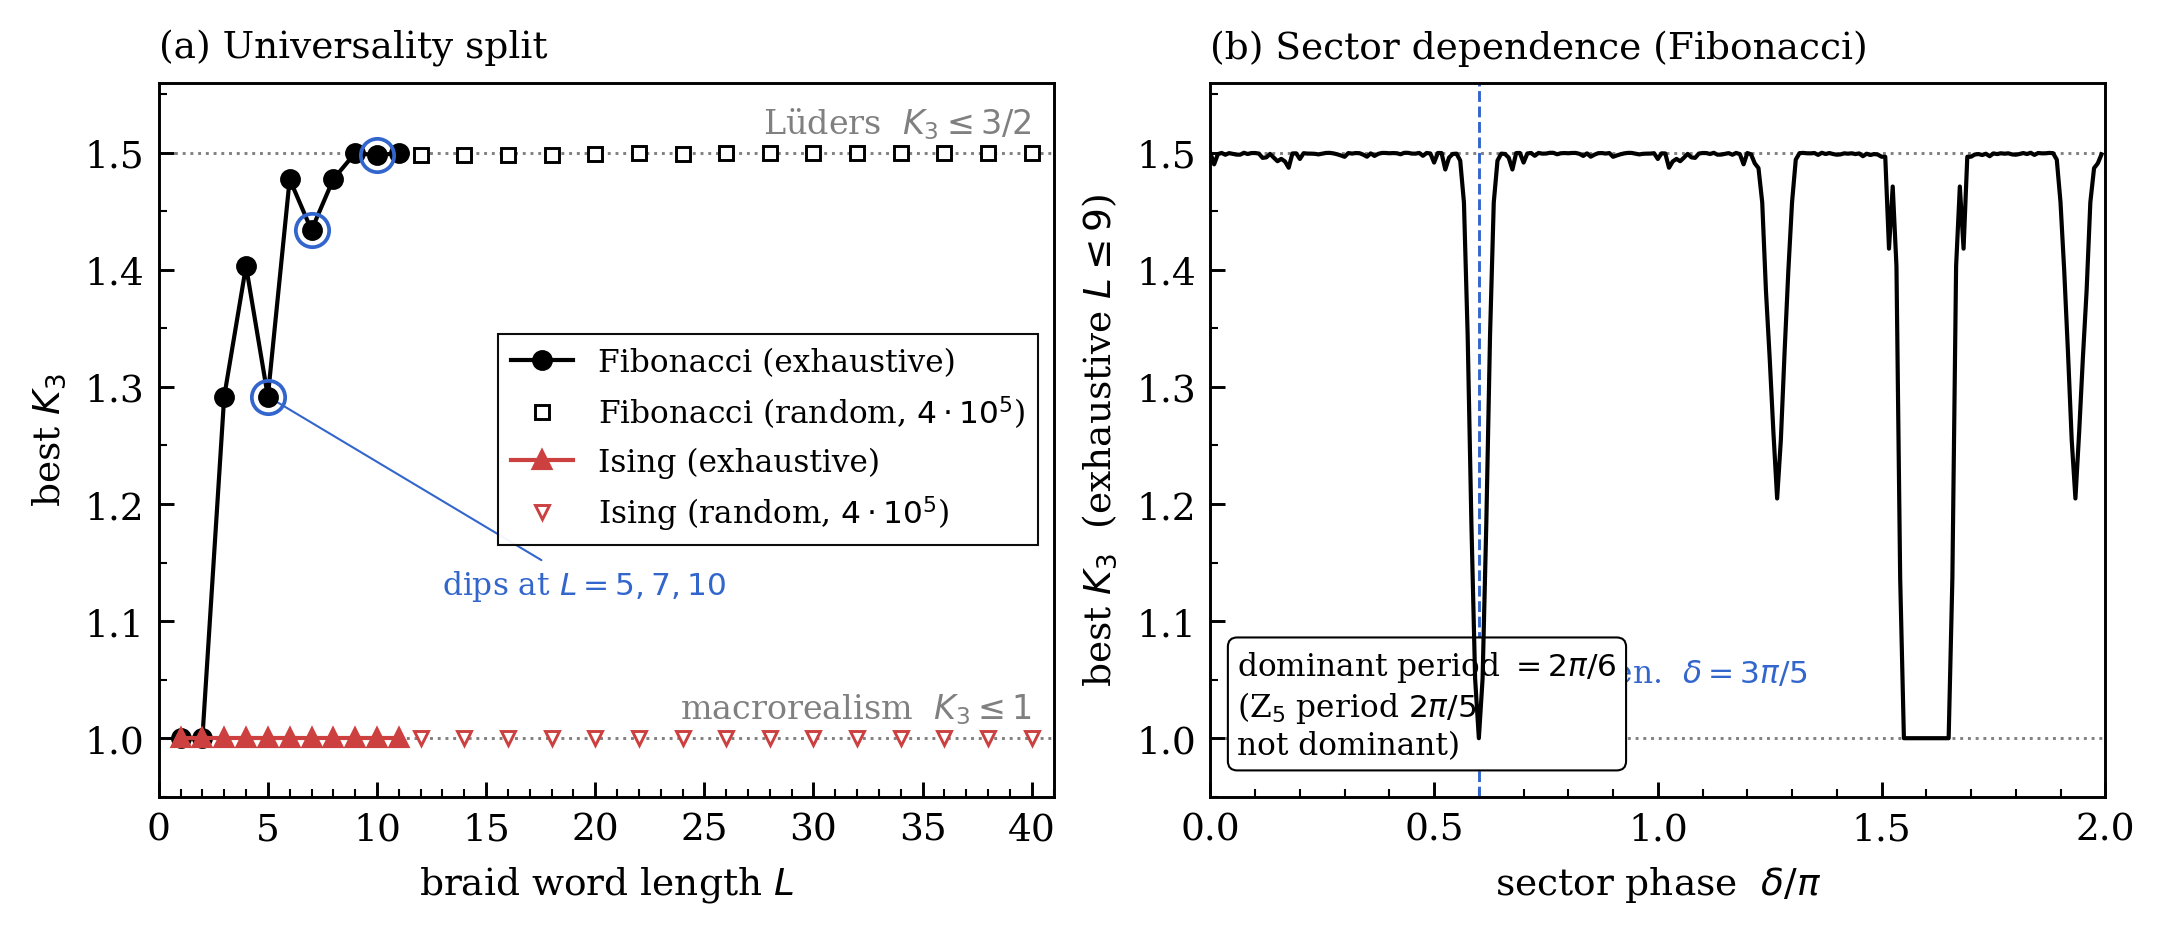
\includegraphics[width=0.95\textwidth]{lgi_letter_figure.png}
\caption{(a)~Best $K_{3}$ versus braid length $L$, $\delta=0$.
\emph{Fibonacci} (black) saturates the L\"uders bound $3/2$ to
$99.998\%$; \emph{Ising} (red) is pinned at $1.0$ for every $L$ tested
(exhaustive to $L=11$; random sampling, $4\times 10^{5}$ words per
$L$, to $L=40$).
(b)~Best $K_{3}(\delta)$ for Fibonacci, exhaustive $L \leq 9$, fine
sampling. The dominant Fourier harmonic is $k=6$, period $2\pi/6$,
reflecting the six R-matrix insertions per
$(\sigma_{1}\sigma_{2})^{3}$ word; the $\mathrm{Z}_{5}$ period
$2\pi/5$ of the central element is not the dominant mode. The
dashed line marks the algebraic
singularity $\delta = 3\pi/5$ at which $\sigma_{1}$ collapses to a
scalar (numerical scalar-deviation $3.1\times 10^{-16}$).}
\label{fig:main}
\end{figure*}

\subsection{Ising: exact $K_{3} = 1$}
\label{sec:ising}

Repeating the same search with the Ising generators gives a
qualitatively different result: $K_{3} = 1.000000$ for the best word
at \emph{every} $L \leq 11$ in the exhaustive search, and the same
for every random sample at $L \in \{12, 14, \ldots, 40\}$
(Fig.~\ref{fig:main}(a), red). The best Ising words realize
$\bigl(C(B),\, C(B^{2})\bigr) = (1,\,1)$ for $L \leq 10$ (the
generators act as $\pm Z$ on the chosen basis), and $(0,\,-1)$ at
$L=11$ (the generators map to $\pm X$), both of which give
$K_{3} = 1$ exactly.

This is the temporal counterpart of the Hou--Shtengel
result~\cite{HouShtengel2016} for the spatial CHSH inequality: in both
cases the Ising-braiding subgroup of $\mathrm{SU}(2)$ is too small to
reach the bound. The intuition is the same: density in
$\mathrm{SU}(2)$ is a necessary condition for saturating the L\"uders
$3/2$ bound by braiding alone, just as it is necessary for saturating
the Tsirelson $2\sqrt{2}$ bound by braiding alone. Ising braiding
generates only Clifford gates and is missing a non-Clifford direction.

\paragraph{Cross-check against a search-space artefact.}
A clean $K_{3}=1.000000$ over $L=1,\ldots,40$ raises the natural
question whether the search has simply missed a violating word. To
rule this out, we apply the same exhaustive procedure to the
Ising generators at deformed sector phases $\delta \neq 0$ (an
algebraic generalization in which the second R-symbol is rotated to
$R_{\psi}\,e^{i\delta}$). The result is that the same code, same
exhaustive depth $L \leq 9$, and same word alphabet recovers
$K_{3}$ values across the full range $[1.000,\,1.500]$ as $\delta$
varies, with $K_{3} = 1.500$ reached at $\delta/\pi \approx 1.167$.
A search that cannot find $K_{3} > 1$ at $\delta = 0$ is therefore
not search-limited; it is genuinely the standard Ising algebra that
forbids the violation. (We do not interpret $\delta \neq 0$ Ising as
a physical model; it is used here only as a falsification probe of
the search procedure.)

We emphasize that the $K_{3} = 1$ result is a statement about the
present two-measurement-step protocol on $\sigma$-anyon braiding
alone. A hybrid protocol that inserts an explicit non-Clifford
resource into an Ising platform---or that uses an Ising-anyon
implementation of a different gate set---could lift $K_{3}$ above $1$.
The result above is for pure braiding within the standard Ising
fusion sector.

\subsection{The scalar singularity at $\delta = 3\pi/5$}

The sector phase $\delta$ rotates $R_{\tau}$ along the unit circle.
At the specific point $\delta_{\star} = 3\pi/5$, the two diagonal
entries of $\sigma_{1}$ coincide:
$R_{\tau} \, e^{i\delta_{\star}}
   = e^{3\pi i/5} \, e^{3\pi i/5}
   = e^{6\pi i/5}
   = R_{1}$,
so $\sigma_{1}$ becomes a scalar times the identity. By
$\sigma_{2} = F \sigma_{1} F$ and $F^{2} = I$, $\sigma_{2}$ then
collapses to the same scalar; every braid word is a global phase, and
no $K_{3} > 1$ is achievable for any $L$. We verify this numerically:
$\|\sigma_{1}(\delta_{\star}) - e^{i\theta}\,I\| = 3.1 \times 10^{-16}$.
This is a clean, exact, machine-precision sub-result that follows
from the algebra of the F- and R-symbols alone.

\subsection{Sector dependence and Fourier period}

Outside the singularity, exhaustive search with $L \leq 9$ explores
the full sector axis (Fig.~\ref{fig:main}(b)). The range of best
$K_{3}$ at fixed budget is $[1.0,\, 1.5]$, with $K_{3} = 1$ reached
also at non-singular $\delta$ values where the required braid is
simply too long for $L \leq 9$: random sampling at the weakest such
sector ($\delta/\pi = 1.556$) with $L = 24$ recovers $K_{3} =
1.4999996$. The $K_{3} = 1$ floor at $L \leq 9$ is therefore a
braid-budget effect, not a sector exclusion. The only true sector
exclusion is the algebraic singularity above.

The Fourier spectrum of $K_{3}(\delta)$ is dominated by $k=6$, i.e.\
period $2\pi/6 = \pi/3$, with amplitude markedly above the secondary
harmonics ($k=2, 4, 1, 12$). The $2\pi/6$ period has a direct
algebraic origin: the central word $(\sigma_{1}\sigma_{2})^{3}$
consists of six generator insertions, each of which carries the
sector phase $\delta$ once through $R_{\tau} \mapsto R_{\tau}\,e^{i\delta}$,
so any quantity invariant under $\delta \mapsto \delta + 2\pi/6$
is preserved. The structurally expected $\mathrm{Z}_{5}$ harmonic
(period $2\pi/5$, corresponding to the central element
$(\sigma_{1}\sigma_{2})^{3}$ as a scalar of order $5$) is
\emph{not} the dominant mode of $K_{3}(\delta)$. We do not
analyze this further here.

\subsection{Initial-state independence}

Equation~(\ref{eq:correlator}) uses the maximally mixed initial state.
We have repeated $K_{3}$ for the optimal $L=11$ word with pure initial
states $|0\rangle$, $|1\rangle$, $|\pm\rangle$, $|\pm i\rangle$, and
three Haar-random pure states. All nine give the same value to
machine precision:
\begin{center}\small
\begin{tabular}{lcc}
\toprule
initial state & $K_{3}$ & spread \\
\midrule
$|0\rangle,\ |1\rangle,\ |\pm\rangle,\ |\pm i\rangle$
              & $1.499762$ & --- \\
$3$ Haar-random pure $|\psi\rangle$
              & $1.499762$ & --- \\
\midrule
mean over pure states & $1.499762$ &
        $|\text{mean}-\text{mixed}| = 0$ \\
\bottomrule
\end{tabular}
\end{center}
This says the L\"uders-saturating value is a property of the
generators themselves: $Z\,U\,Z\,U^{\dagger}$ and $Z\,U^{2}\,Z\,(U^{2})^{\dagger}$
are proportional to the identity for the optimal $U$, so every pure
state gives the same expectation value. The saturation is algebraic,
not state-engineered. This pre-empts a natural reviewer concern that
the mixed-state convention might mask a more nuanced state dependence.

\section{Discussion}
\label{sec:discussion}

\paragraph{What the universality split says.}
The pair (Fibonacci, Ising) is the natural minimal test bed for
universality-driven phenomena in non-abelian anyon platforms.
Hou and Shtengel~\cite{HouShtengel2016} established that
Ising-braiding alone cannot violate the spatial CHSH inequality
(Tsirelson saturation requires a non-Clifford gate), while the
universal Fibonacci model
saturates~\cite{Brennen2009,NayakSimonStern2008}. The present results
show that the same split holds for the \emph{temporal} inequality:
Fibonacci saturates the L\"uders bound to $99.998\%$ while Ising is
pinned at $1.0$. In a single sentence: universality is the property
that allows a non-abelian anyon braid to saturate both the spatial
and the temporal projective-quantum bounds.

\paragraph{What it does not say.}
The Fibonacci L\"uders saturation is not, by itself, evidence for a
non-classical \emph{topological} mechanism beyond what the modular
tensor category already prescribes. Fibonacci density in
$\mathrm{SU}(2)$ guarantees that any unitary---including the one
realizing the L\"uders-saturating product---can be approximated by a
braid word; the role of topology here is to provide that universal
gate set, not to add an additional non-classical resource. The
Leggett--Garg saturation is a TQFT-consistency demonstration, in the
same sense in which the spatial CHSH saturation is a TQFT-consistency
demonstration. The interest of the result lies in (i) closing the
non-abelian Bell/Leggett--Garg literature gap, (ii) the sharpness of
the Fibonacci/Ising split, and (iii) the three structural signatures
(scalar singularity, period match, state independence) that are not
implied by universality alone.

\paragraph{Relation to G\'omez-Ruiz~\textit{et~al.}~2018.}
G\'omez-Ruiz \emph{et al.}~\cite{GomezRuiz2018} test the three-time
LGI in the form $K_{i,j}(t) = 2\,C_{i,j}(t) - C_{i,j}(2t) \leq 1$ on
Dirac qubits formed from edge Majorana modes of the Kitaev chain.
That system is abelian; the test serves as a probe of the topological
phase transition. Their maximum reported violation $K_{\rm Max}(\mu)$
reaches $\approx 1.5$ across a chemical-potential sweep but is not
analyzed as a saturation distance to the L\"uders bound. The present
work tests $K_{3}$ on the non-abelian fusion-channel qubit of three
$\tau$ anyons; the Fibonacci-Ising universality split is the central
comparison; and the saturation is reported as a $3.6 \times 10^{-5}$
gap to the L\"uders bound (i.e.\ $99.998\%$) obtained by braid-word
optimization, rather than as a transition diagnostic. Both works
belong to the genre ``Leggett--Garg on a topological system''; they
are methodologically and physically distinct sub-cases.

\paragraph{What an experiment would look like.}
A direct test requires (i) a platform supporting non-abelian
braiding---present candidates are filling-fraction $\nu = 12/5$ for
Fibonacci~\cite{NayakSimonStern2008} and quantum-processor
implementations of Fibonacci string-nets~\cite{Xu2024,Minev2025};
(ii) projective measurement of the fusion channel of an anyon
pair~\cite{Bonderson2008}; (iii) the ability to apply a deterministic
braid word between measurements. The Hou--Shtengel split predicts
that on any Ising-anyon platform~\cite{Andersen2023,Iqbal2024} the
$K_{3}$ would be pinned at $1$ even in the absence of decoherence.
The robustness of $K_{3}$ to depolarizing noise on the platform
benchmark of~\cite{Andersen2023} would have to be analyzed
separately.

\section{Open questions}
\label{sec:open}

Three natural extensions are immediate but outside the scope of this
note:
\begin{enumerate}
\item[\textbf{O1.}] $K_{n}$ for $n > 3$. The L\"uders bound increases
toward the algebraic limit $K_{n} \to n$ with $n$. Does
Fibonacci-braiding saturate the moving bound at each $n$? A
multi-time Leggett--Garg test with $n=4,5,\ldots$ is a one-day
extension of the present setup.
\item[\textbf{O2.}] Structural origin of the non-monotonicity dips.
The dips at $L = 5, 7, 10$ in the present LGI data should encode the
divisibility structure of the central element $(\sigma_{1}\sigma_{2})^{3}$
of $B_{3}$. A systematic correlation of dip-position with the algebra
is a sharper version of ``best at length $L$'' than the running
maximum.
\item[\textbf{O3.}] Representation dependence of the temporal bound.
Sorella~\cite{Sorella2023} has argued that the spatial Tsirelson
bound is representation-dependent in dimensions higher than two. The
temporal counterpart---whether the L\"uders bound $3/2$ is
representation-dependent in $\dim > 2$ fusion spaces---is open. Our
setup is fixed at $\dim = 2$; a $\dim > 2$ extension would address
this directly.
\end{enumerate}

\section{Code and data}

All code and result files are released with this preprint under
\href{https://creativecommons.org/licenses/by/4.0/}{CC~BY~4.0}.
Reproduction is deterministic with the random seeds
\texttt{20260524} (Fibonacci main and period scan) and
\texttt{20260525} (Ising and pure-state robustness). All
computations use only \texttt{numpy} and \texttt{matplotlib}.
Sanity checks at the head of each script must pass at machine
precision; if they do not, the generator conventions have been
altered.

\begin{thebibliography}{99}

\bibitem{LeggettGarg1985}
A.~J.~Leggett and A.~Garg,
\emph{Quantum mechanics versus macroscopic realism: Is the flux there when nobody looks?}
Phys.\ Rev.\ Lett.\ \textbf{54}, 857 (1985).

\bibitem{Budroni2014}
C.~Budroni and C.~Emary,
\emph{Temporal quantum correlations and Leggett-Garg inequalities in multi-level systems},
Phys.\ Rev.\ Lett.\ \textbf{113}, 050401 (2014).

\bibitem{EmaryLambertNori2014}
C.~Emary, N.~Lambert, and F.~Nori,
\emph{Leggett-Garg inequalities},
Rep.\ Prog.\ Phys.\ \textbf{77}, 016001 (2014).

\bibitem{Fine1982}
A.~Fine,
\emph{Hidden variables, joint probability, and the Bell inequalities},
Phys.\ Rev.\ Lett.\ \textbf{48}, 291 (1982).

\bibitem{NayakSimonStern2008}
C.~Nayak, S.~H.~Simon, A.~Stern, M.~Freedman, and S.~Das~Sarma,
\emph{Non-Abelian anyons and topological quantum computation},
Rev.\ Mod.\ Phys.\ \textbf{80}, 1083 (2008).

\bibitem{Bonderson2008}
P.~Bonderson, M.~Freedman, and C.~Nayak,
\emph{Measurement-only topological quantum computation},
Phys.\ Rev.\ Lett.\ \textbf{101}, 010501 (2008).

\bibitem{HouShtengel2016}
C.-Y.~Hou \emph{et al.},
\emph{Comment on `Topological qubits with Majorana fermions'} and the
underlying Clifford-only structure of Ising braiding,
Phys.\ Rev.\ X \textbf{6}, 021005 (2016).

\bibitem{Brennen2009}
G.~K.~Brennen, S.~Iblisdir, J.~K.~Pachos, and J.~K.~Slingerland,
\emph{Non-locality of non-abelian anyons},
New J.\ Phys.\ \textbf{11}, 103023 (2009);
\href{https://arxiv.org/abs/0810.4319}{arXiv:0810.4319}.

\bibitem{GomezRuiz2018}
F.~J.~G\'omez-Ruiz, J.~J.~Mendoza-Arenas, F.~J.~Rodr\'iguez,
C.~Tejedor, and L.~Quiroga,
\emph{Universal two-time correlations, out-of-time-ordered
correlators and Leggett-Garg inequality violation by edge Majorana
fermion qubits},
Phys.\ Rev.\ B \textbf{97}, 235134 (2018);
\href{https://arxiv.org/abs/1802.10522}{arXiv:1802.10522}.

\bibitem{Sorella2023}
S.~P.~Sorella,
\emph{Representation dependence of the Tsirelson bound},
preprint, \href{https://arxiv.org/abs/2304.05696}{arXiv:2304.05696} (2023).

\bibitem{Andersen2023}
T.~I.~Andersen \emph{et al.} (Google Quantum AI),
\emph{Non-Abelian braiding of graph vertices in a superconducting processor},
Nature \textbf{618}, 264 (2023).

\bibitem{Iqbal2024}
M.~Iqbal \emph{et al.} (Quantinuum),
\emph{Non-Abelian topological order and anyons on a trapped-ion processor},
Nature \textbf{626}, 505 (2024).

\bibitem{Xu2024}
S.~Xu \emph{et al.},
\emph{Non-abelian braiding of Fibonacci anyons with a superconducting processor},
Nat.\ Phys.\ \textbf{20}, 1469 (2024).

\bibitem{Minev2025}
Z.~Minev, S.~Najafi \emph{et al.},
\emph{Realization of a Fibonacci string-net on a quantum processor},
Nat.\ Commun.\ \textbf{16} (2025).

\end{thebibliography}

\end{document}
